%!TEX root = ../TTK4900-MHT.tex

\chapter{Initialization time plot}
\begin{figure}
\centering
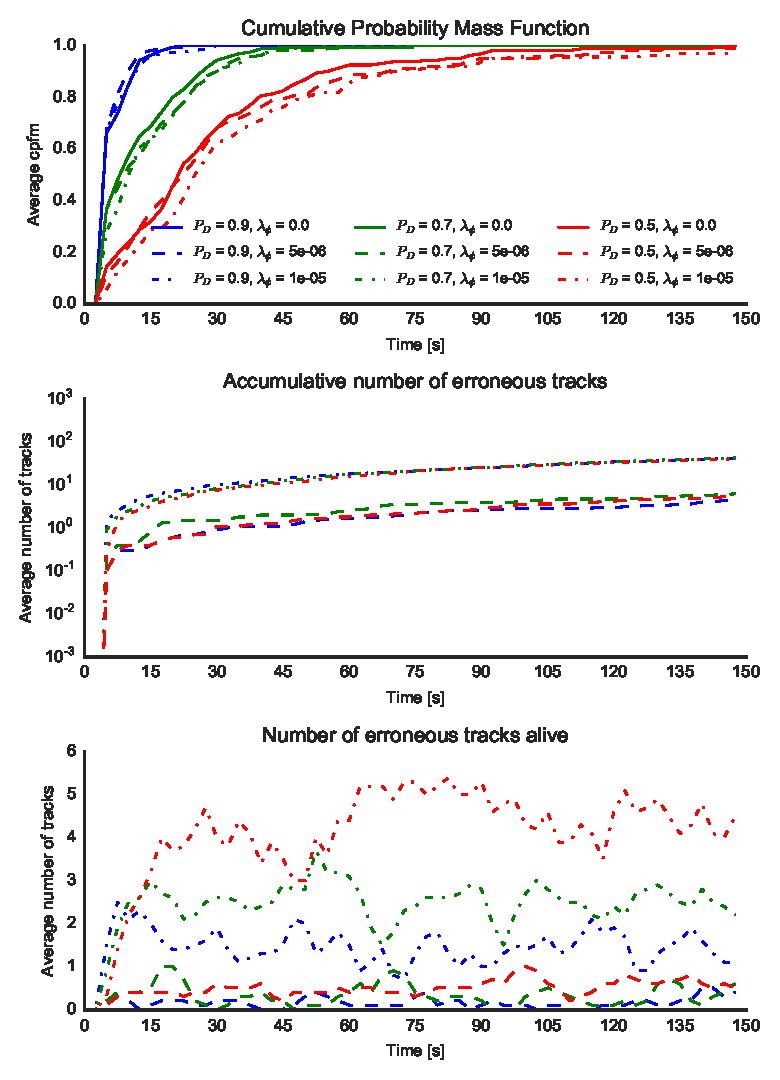
\includegraphics{Figures/plots/Scenario1_Init-Time(1-1).pdf}
\caption{Initialization time (1/1)}\label{fig:init_time_1-1}
\end{figure}

\begin{figure}
\centering
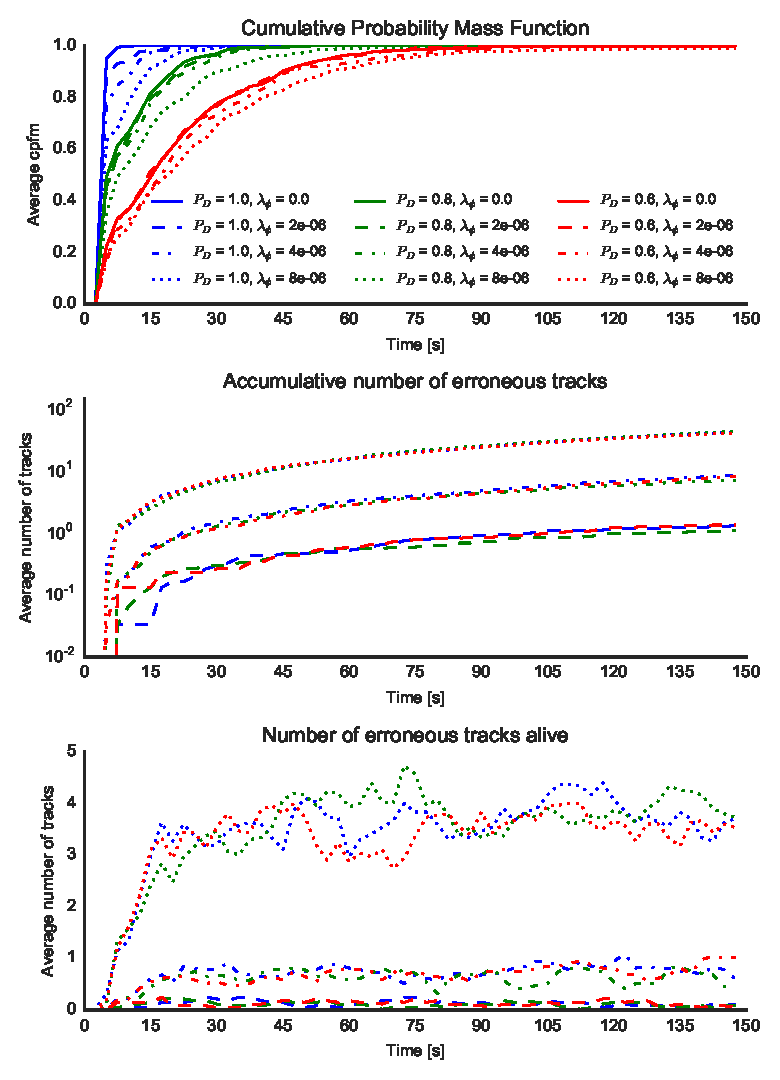
\includegraphics{Figures/plots/Scenario1_Init-Time(1-2).pdf}
\caption{Initialization time (1/2)}\label{fig:init_time_1-2}
\end{figure}

\begin{figure}
\centering
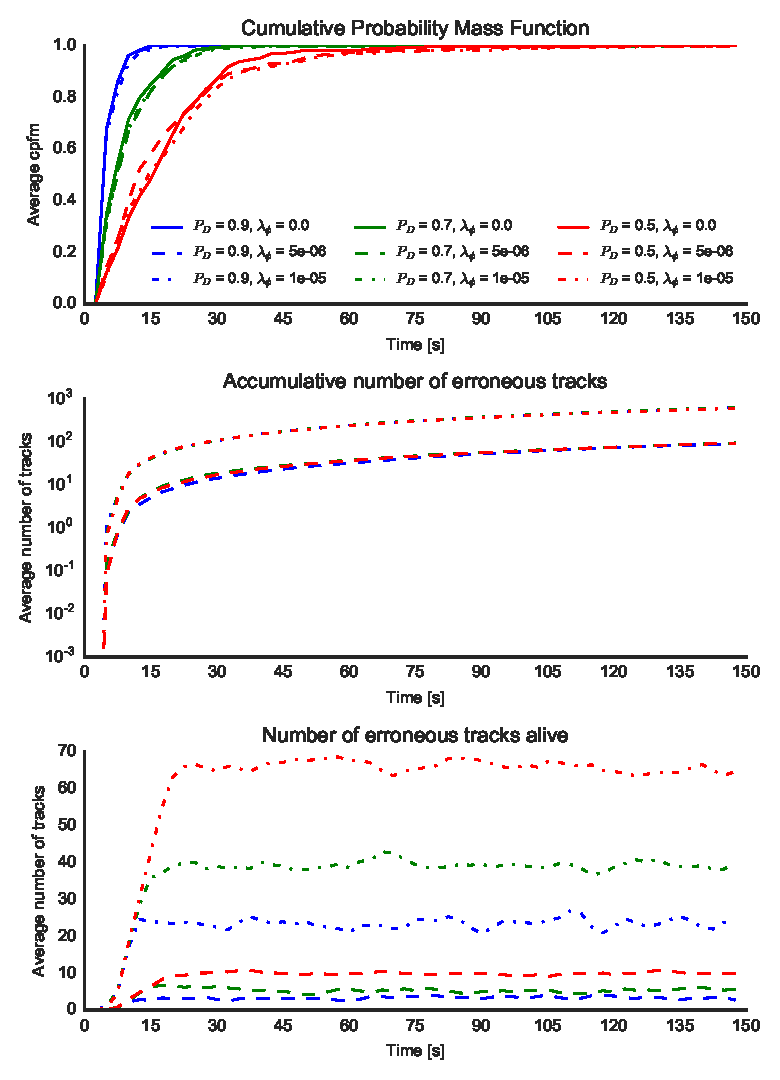
\includegraphics{Figures/plots/Scenario1_Init-Time(1-3).pdf}
\caption{Initialization time (1/3)}\label{fig:init_time_1-3}
\end{figure}

\begin{figure}
\centering
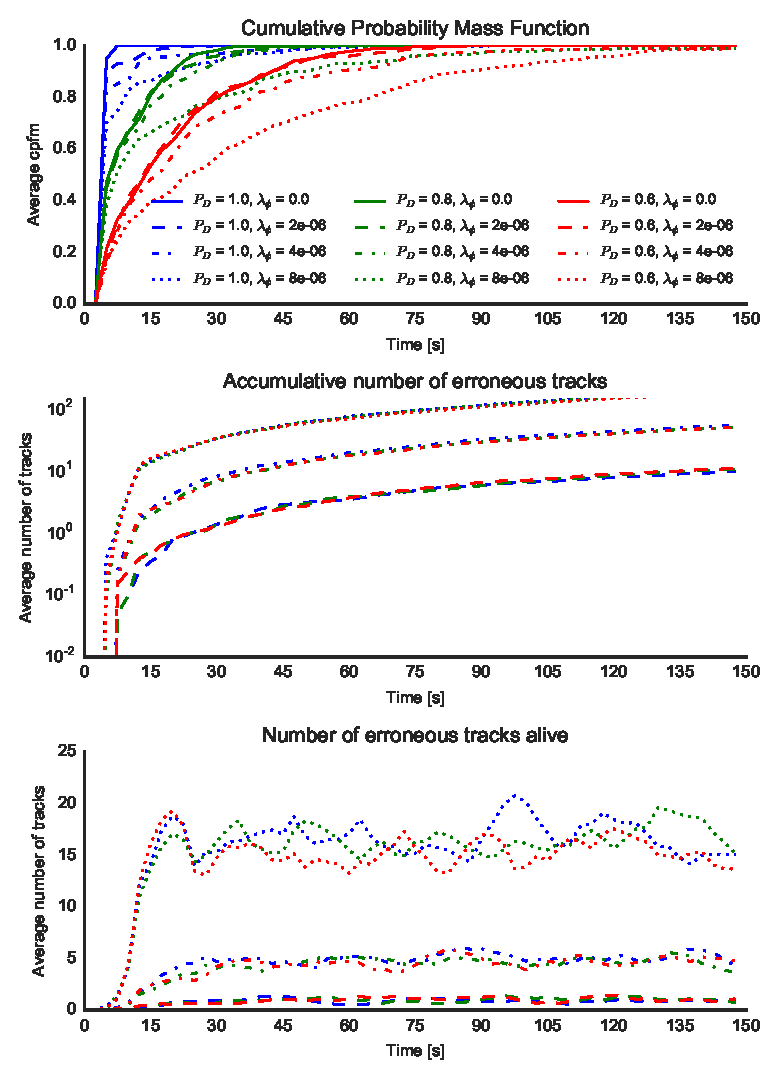
\includegraphics{Figures/plots/Scenario1_Init-Time(1-4).pdf}
\caption{Initialization time (1/4)}\label{fig:init_time_1-4}
\end{figure}

\begin{figure}
\centering
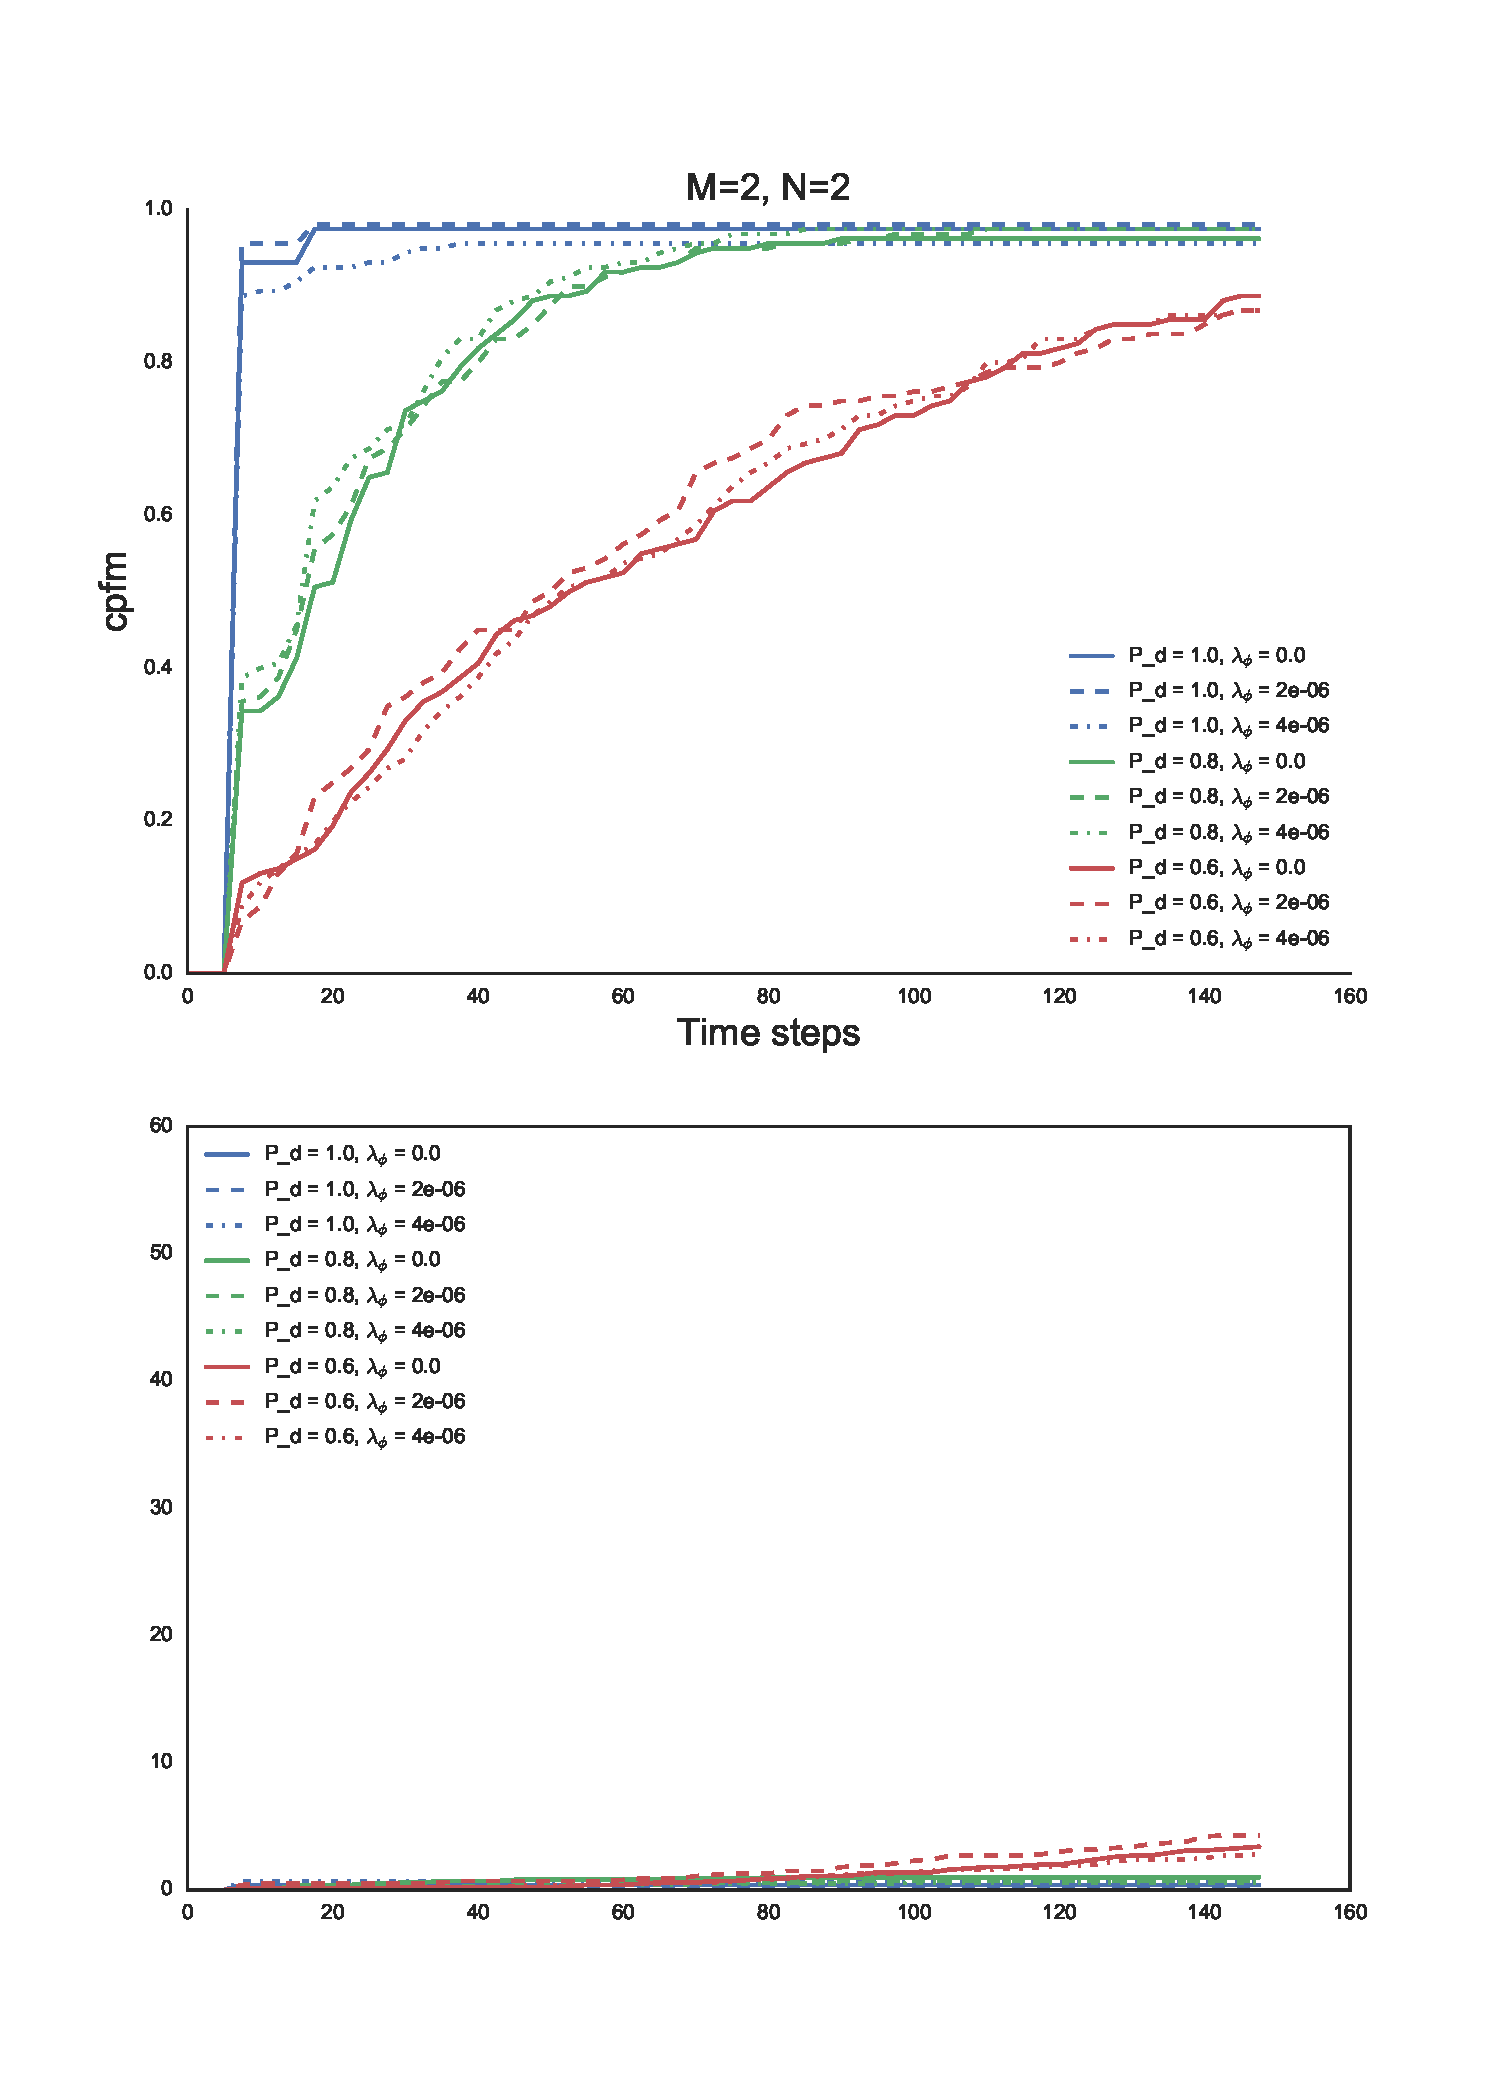
\includegraphics{Figures/plots/Scenario1_Init-Time(2-2).pdf}
\caption{Initialization time (2/2)}\label{fig:init_time_2-2}
\end{figure}

\begin{figure}
\centering
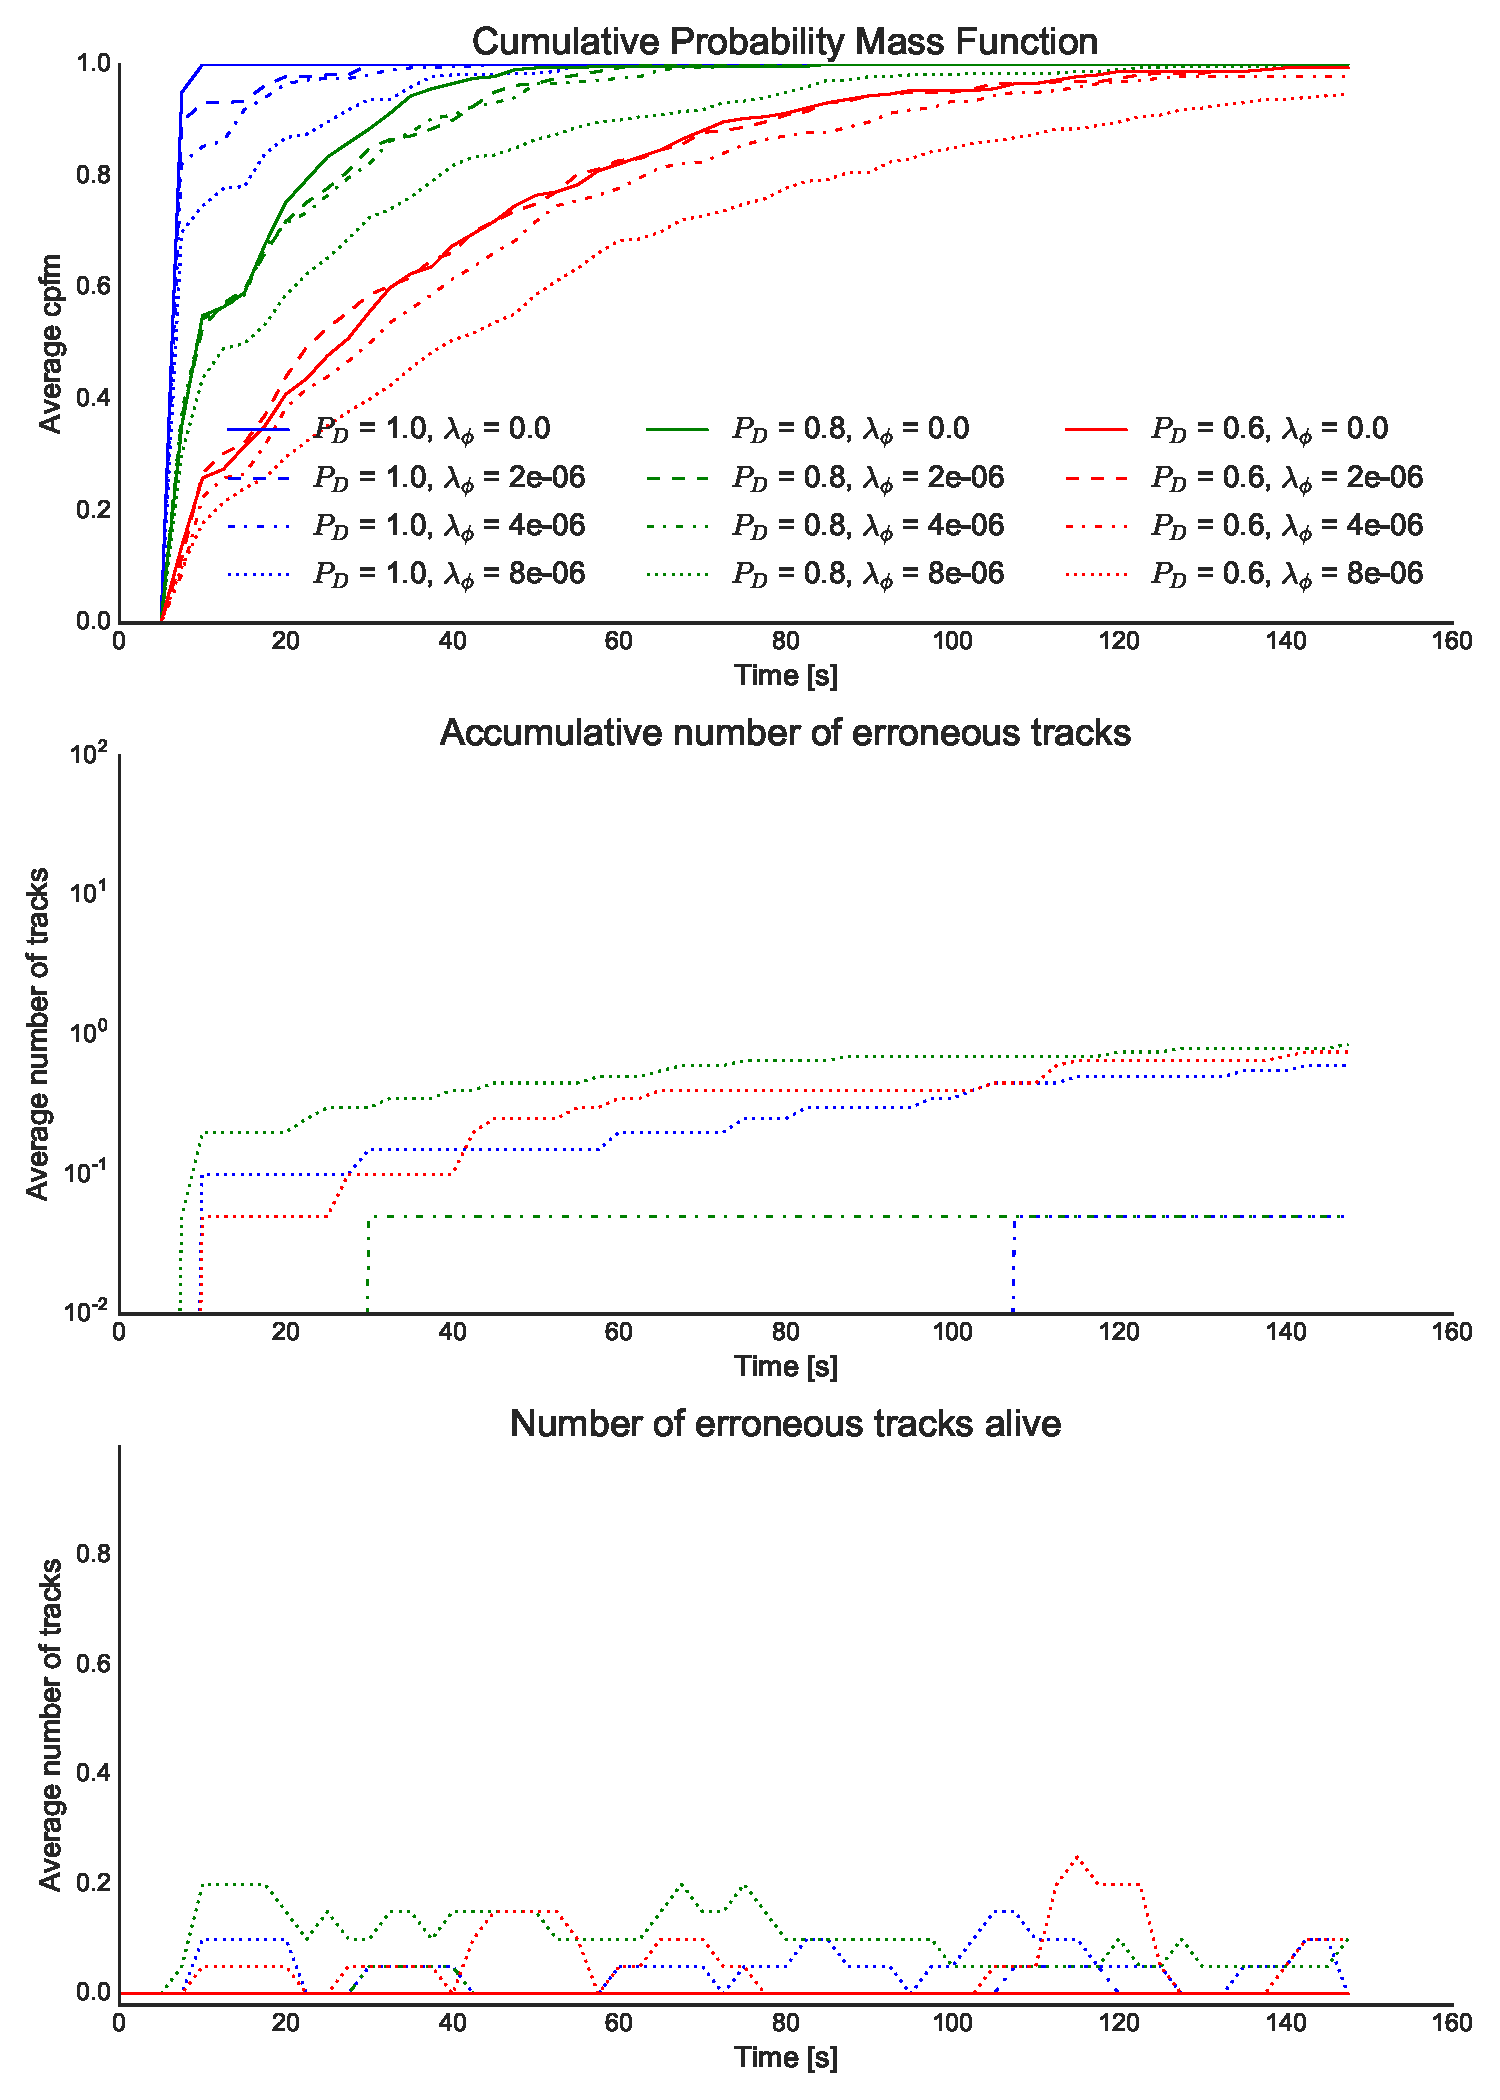
\includegraphics{Figures/plots/Scenario1_Init-Time(2-3).pdf}
\caption{Initialization time (2/3)}\label{fig:init_time_2-3}
\end{figure}

\begin{figure}
\centering
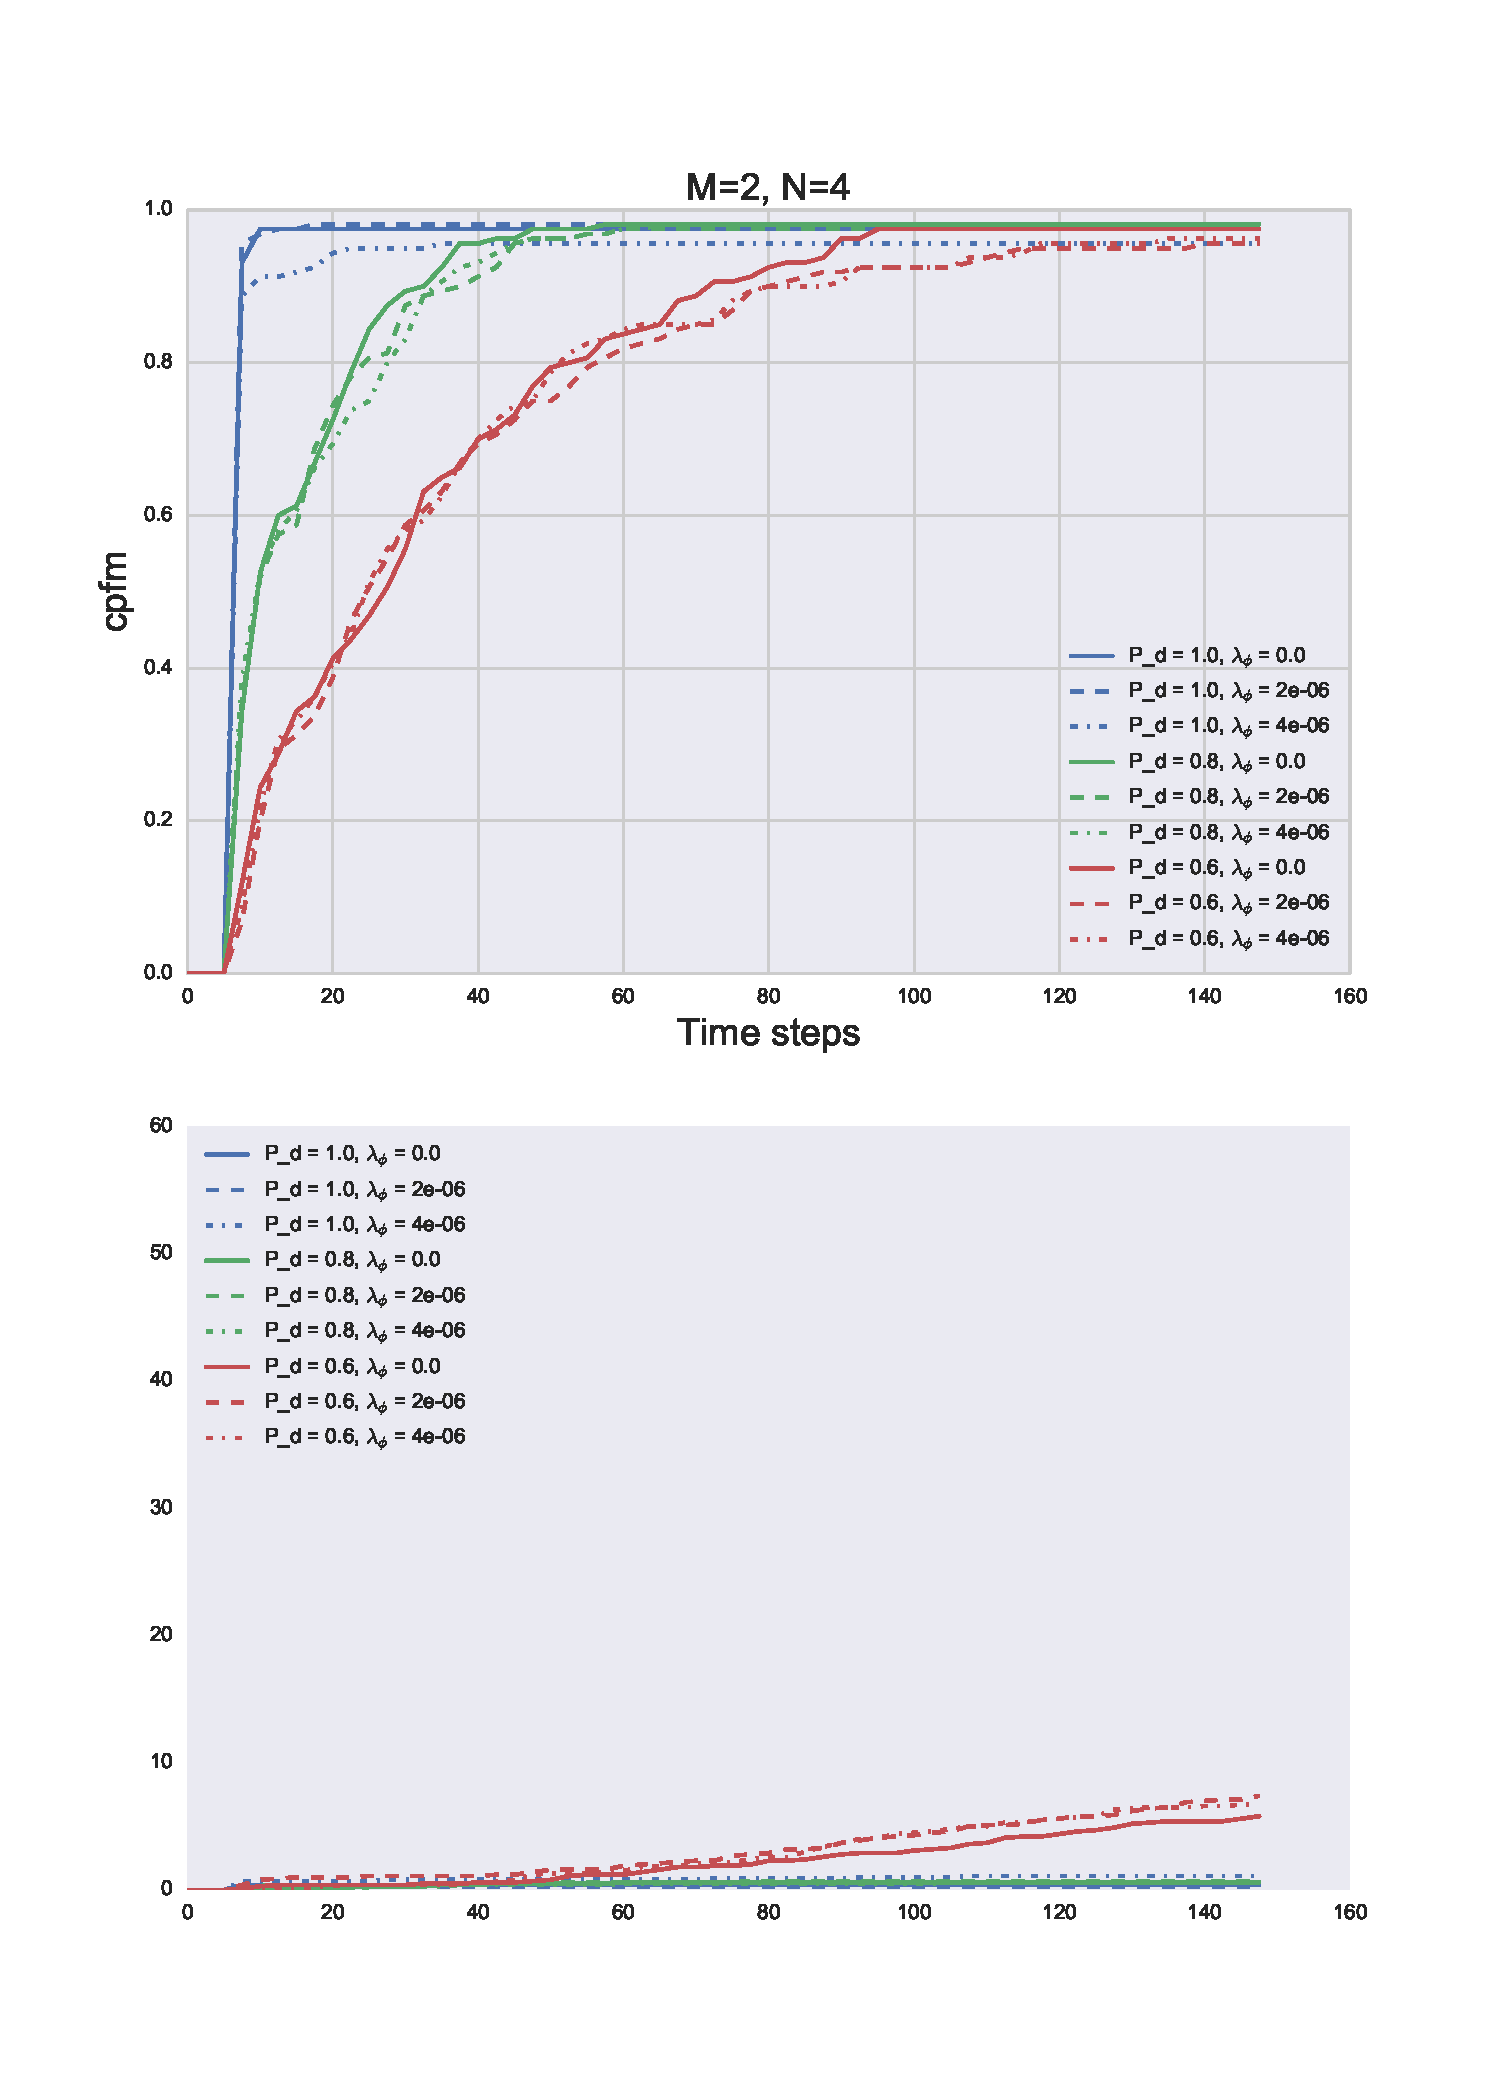
\includegraphics{Figures/plots/Scenario1_Init-Time(2-4).pdf}
\caption{Initialization time (2/4)}\label{fig:init_time_2-4}
\end{figure}

\begin{figure}
\centering
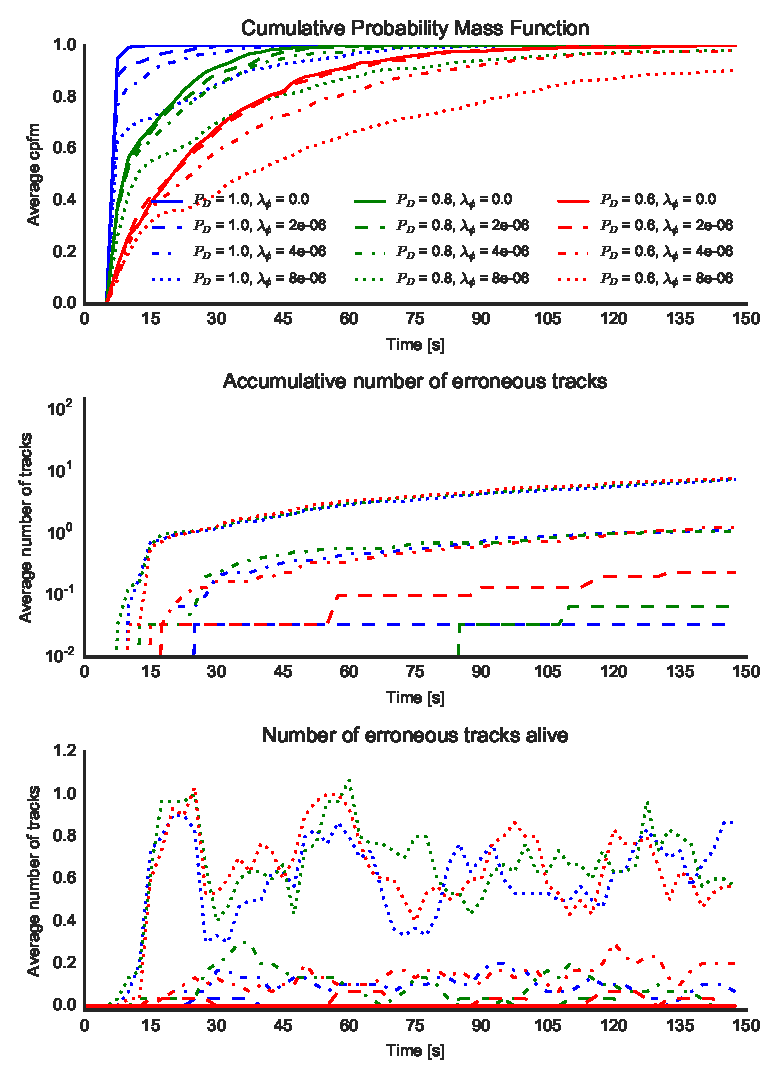
\includegraphics{Figures/plots/Scenario1_Init-Time(2-5).pdf}
\caption{Initialization time (2/5)}\label{fig:init_time_2-5}
\end{figure}

\begin{figure}
\centering
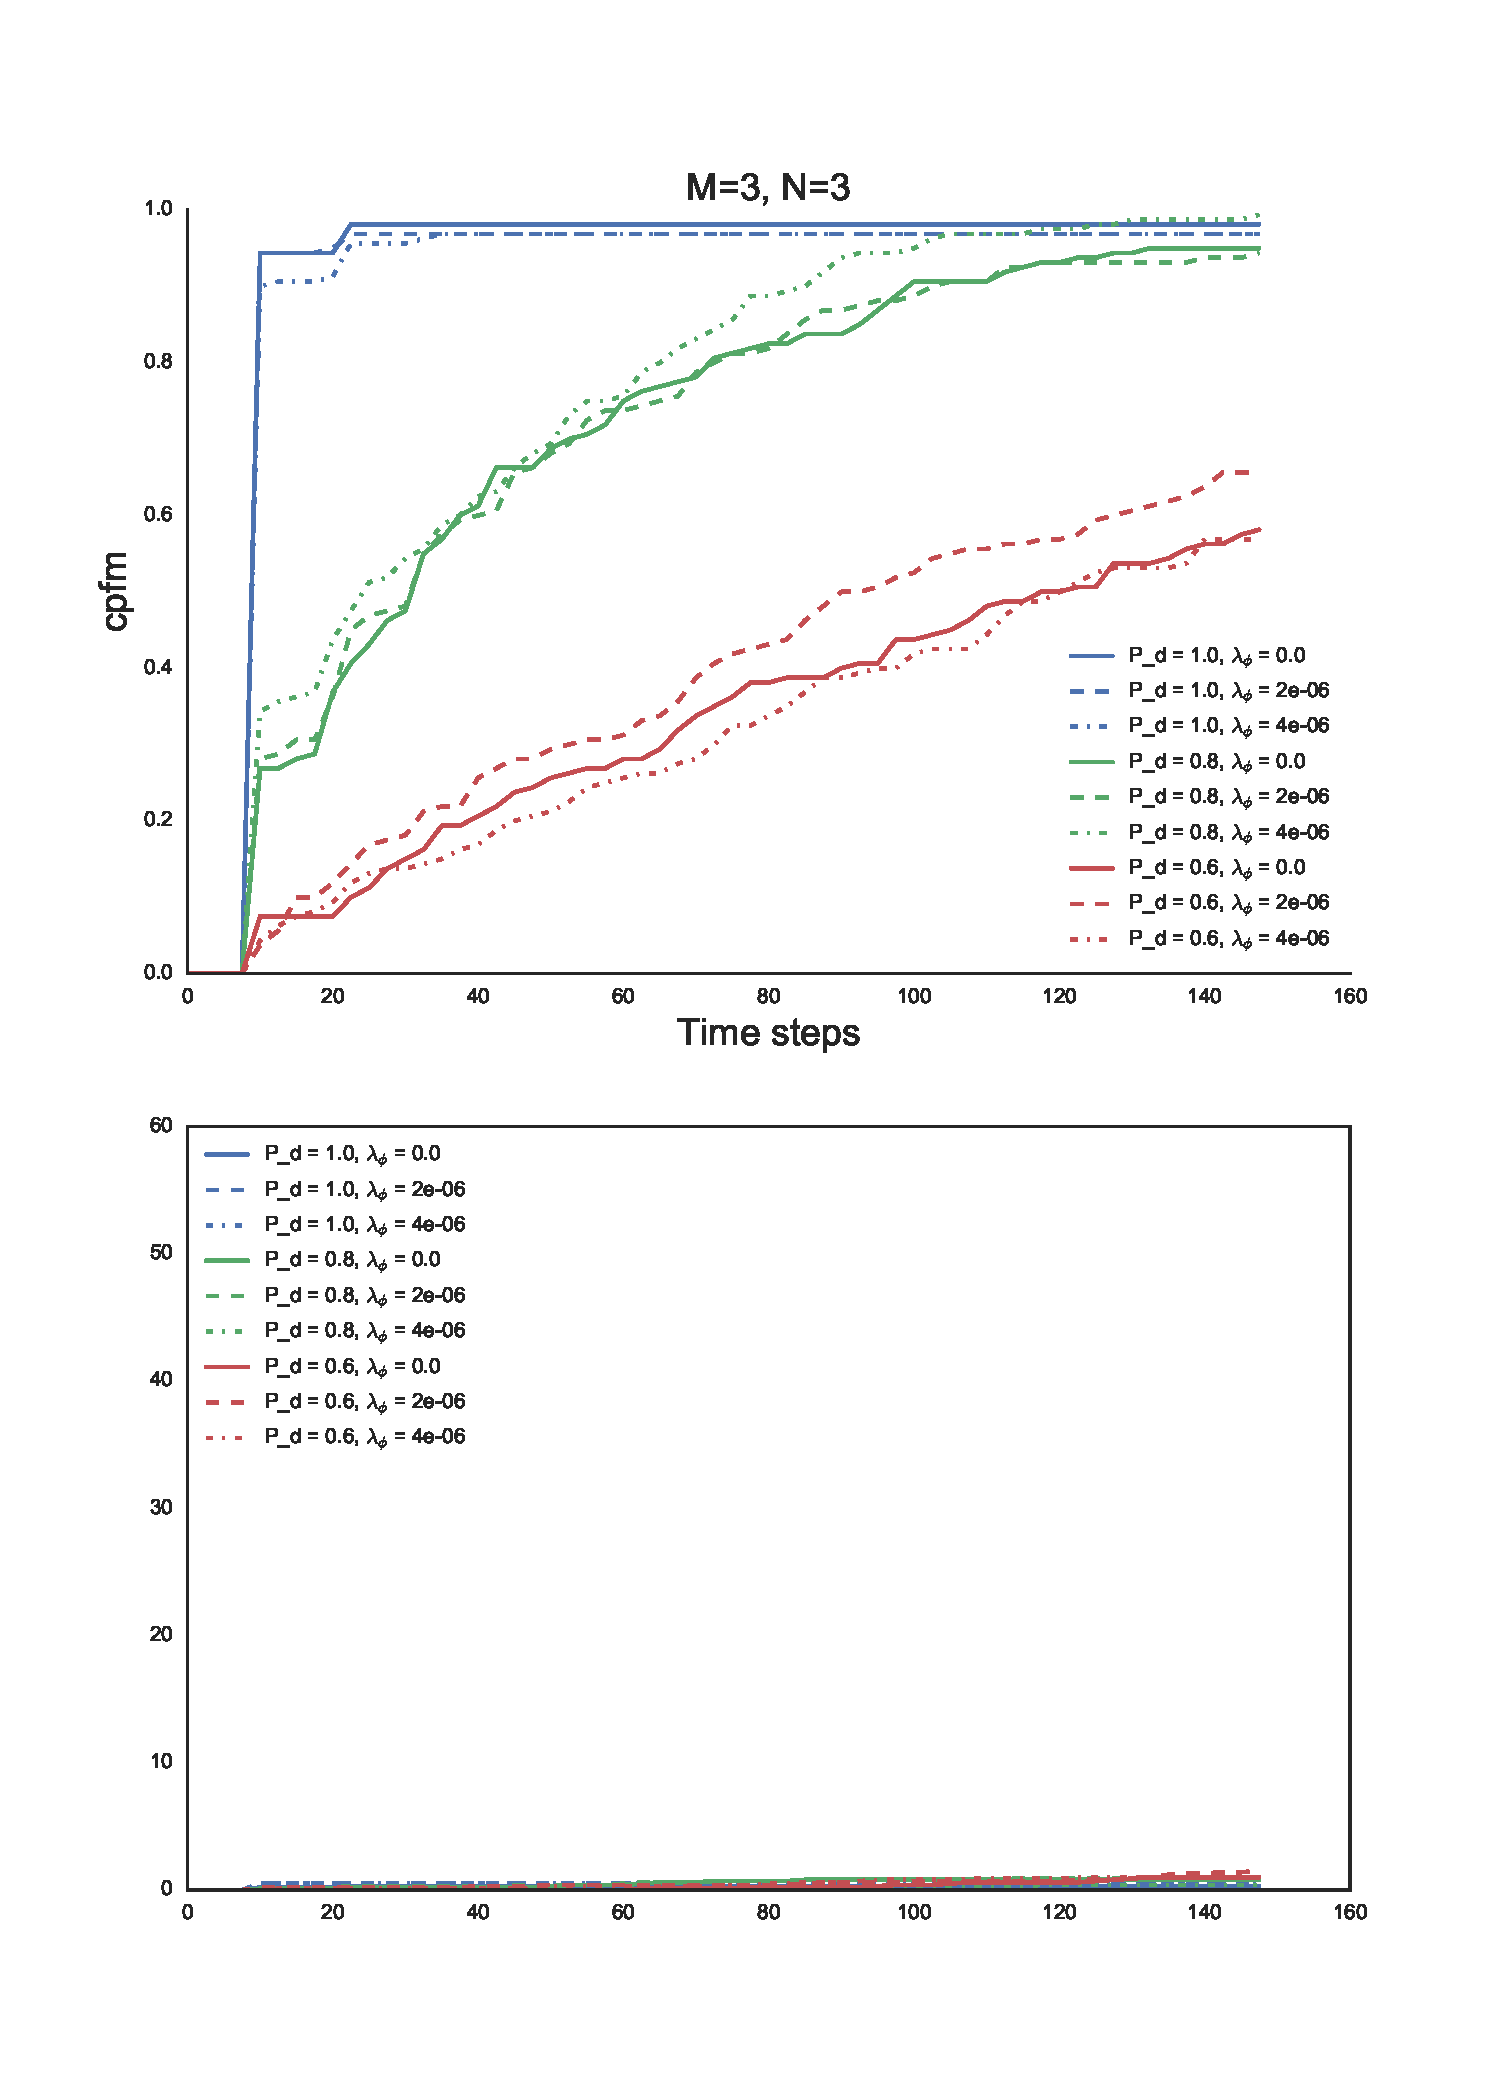
\includegraphics{Figures/plots/Scenario1_Init-Time(3-3).pdf}
\caption{Initialization time (3/3)}\label{fig:init_time_3-3}
\end{figure}

\begin{figure}
\centering
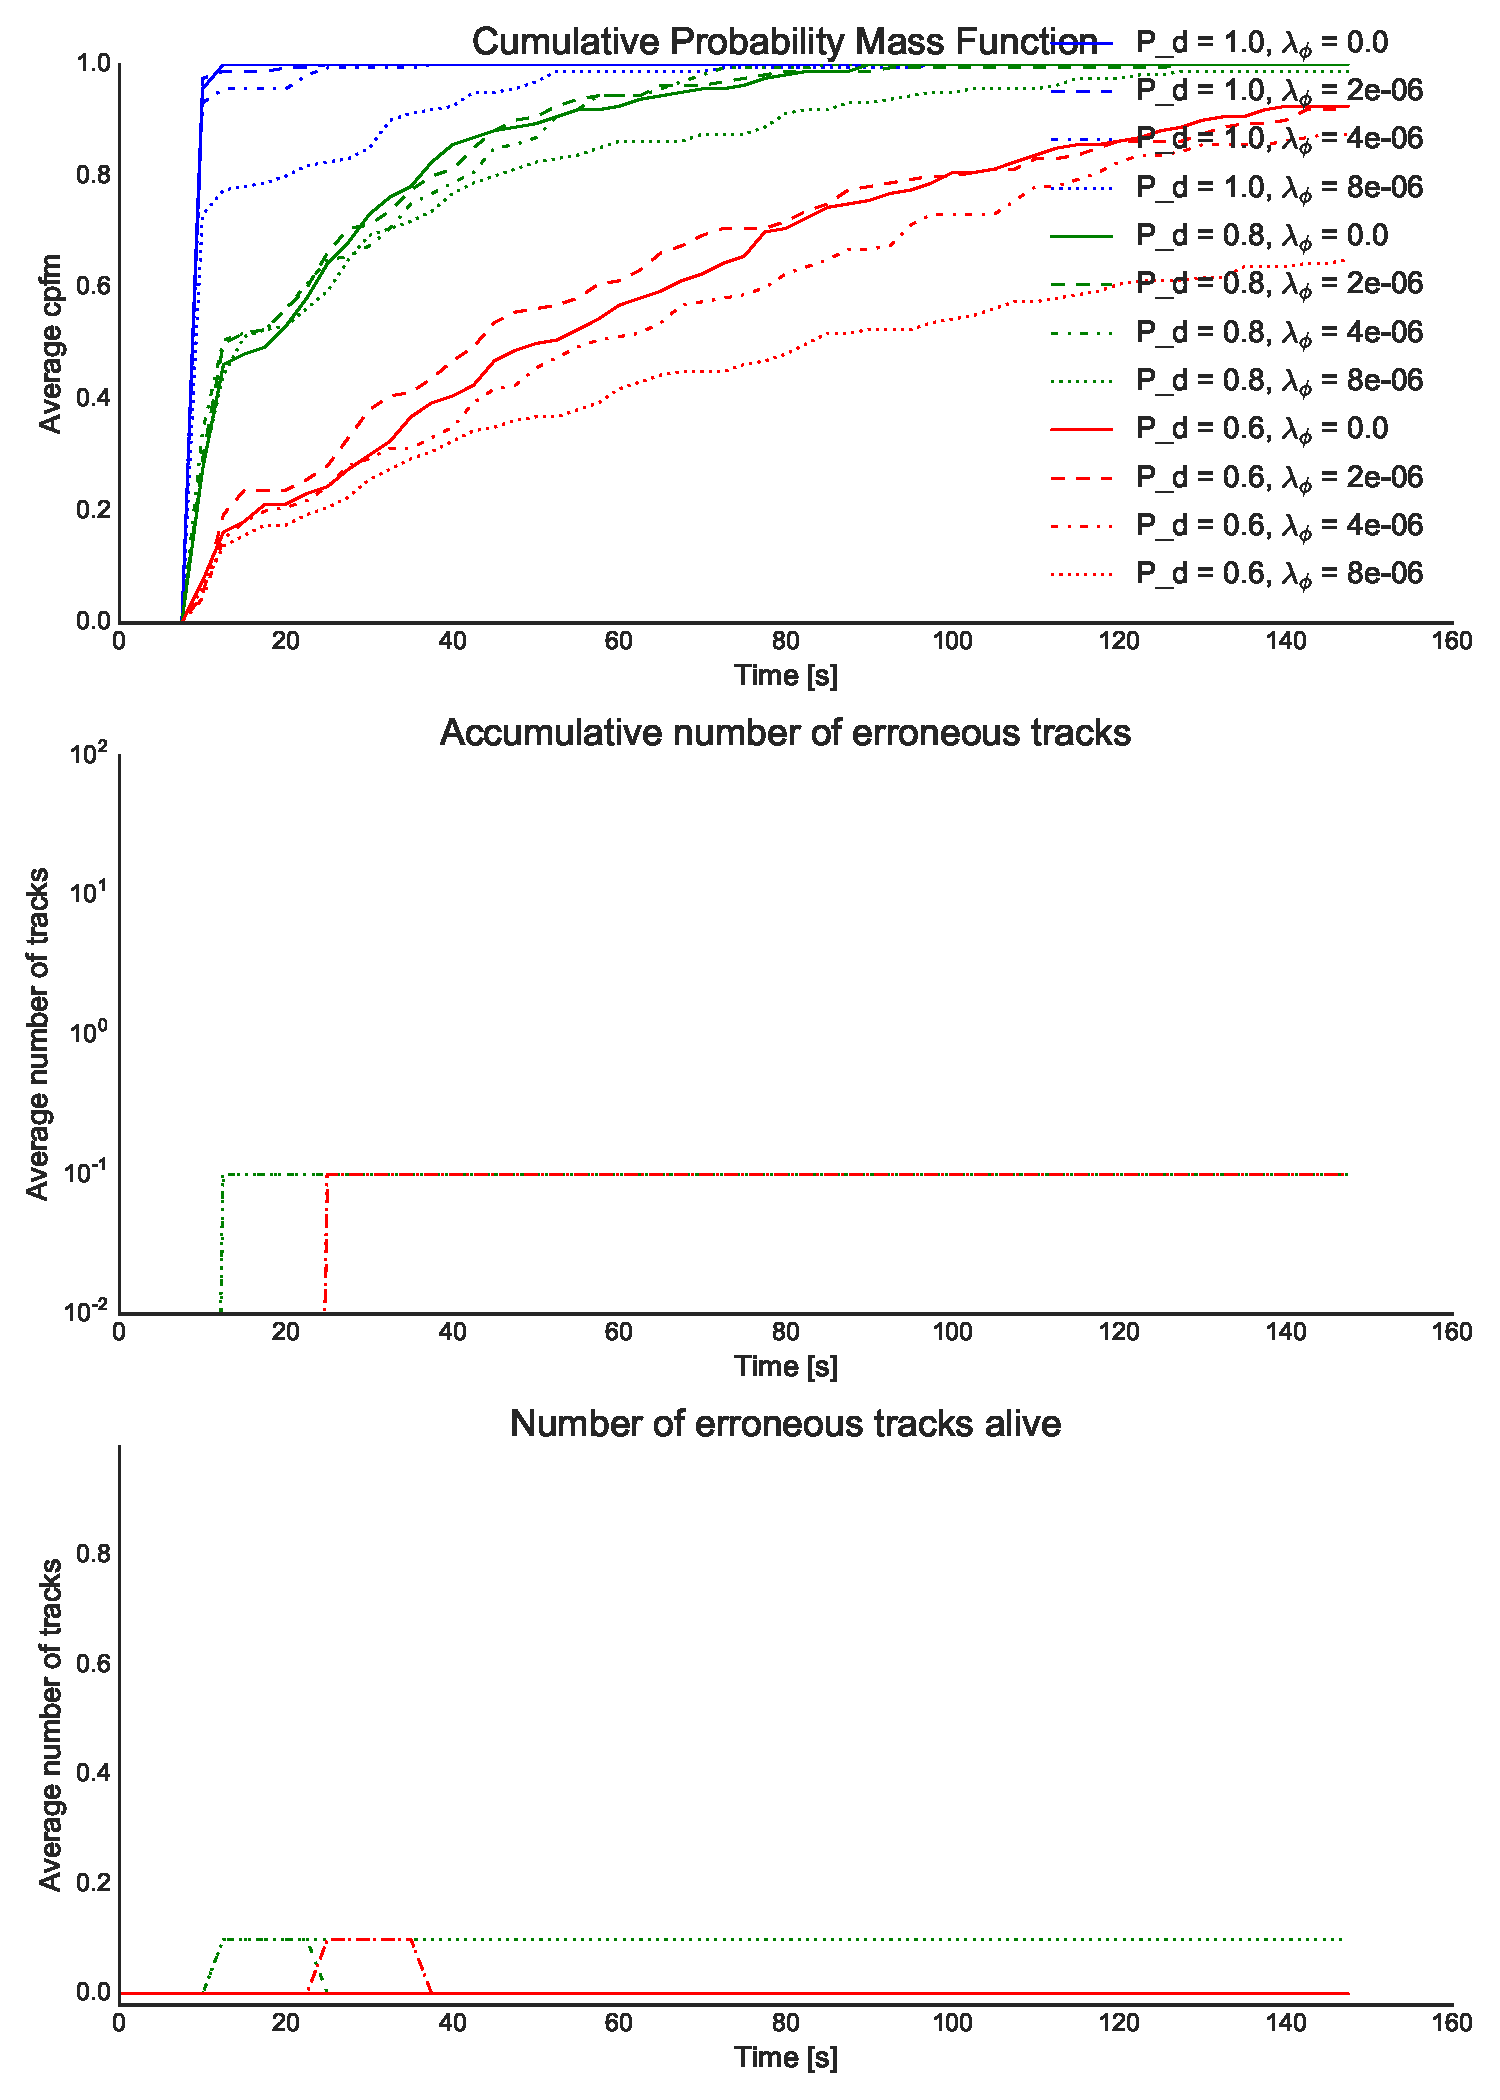
\includegraphics{Figures/plots/Scenario1_Init-Time(3-4).pdf}
\caption{Initialization time (3/4)}\label{fig:init_time_3-4}
\end{figure}

\begin{figure}
\centering
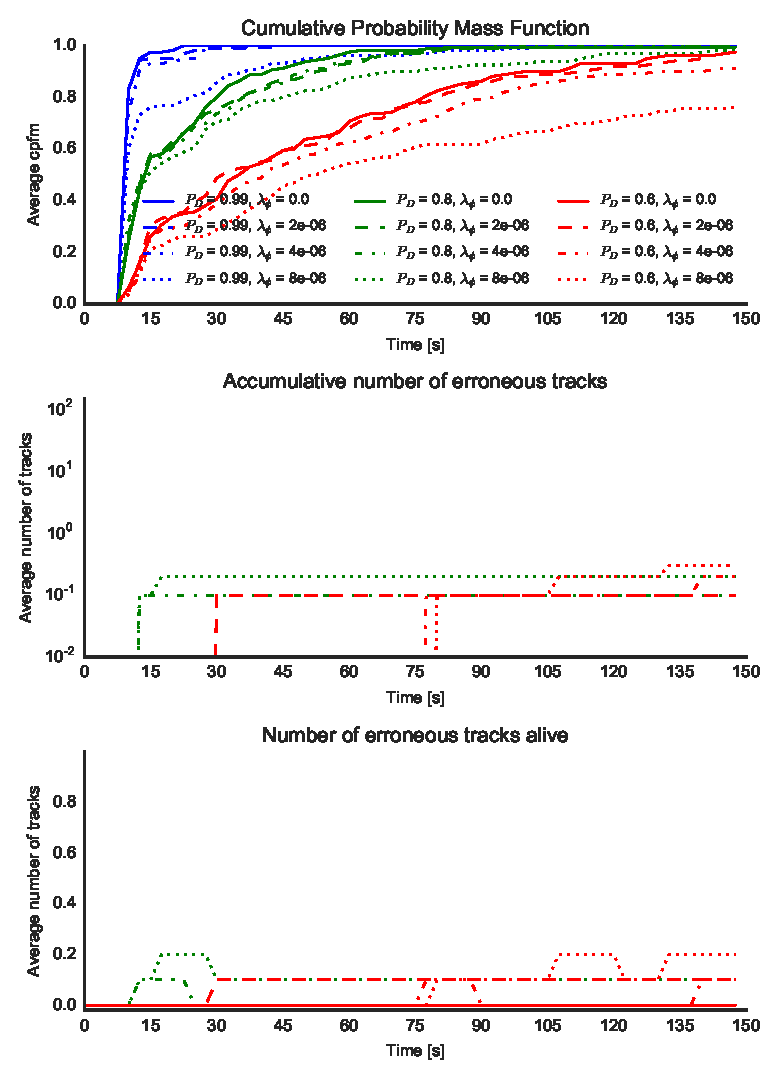
\includegraphics{Figures/plots/Scenario1_Init-Time(3-5).pdf}
\caption{Initialization time (3/5)}\label{fig:init_time_3-5}
\end{figure}

\begin{figure}
\centering
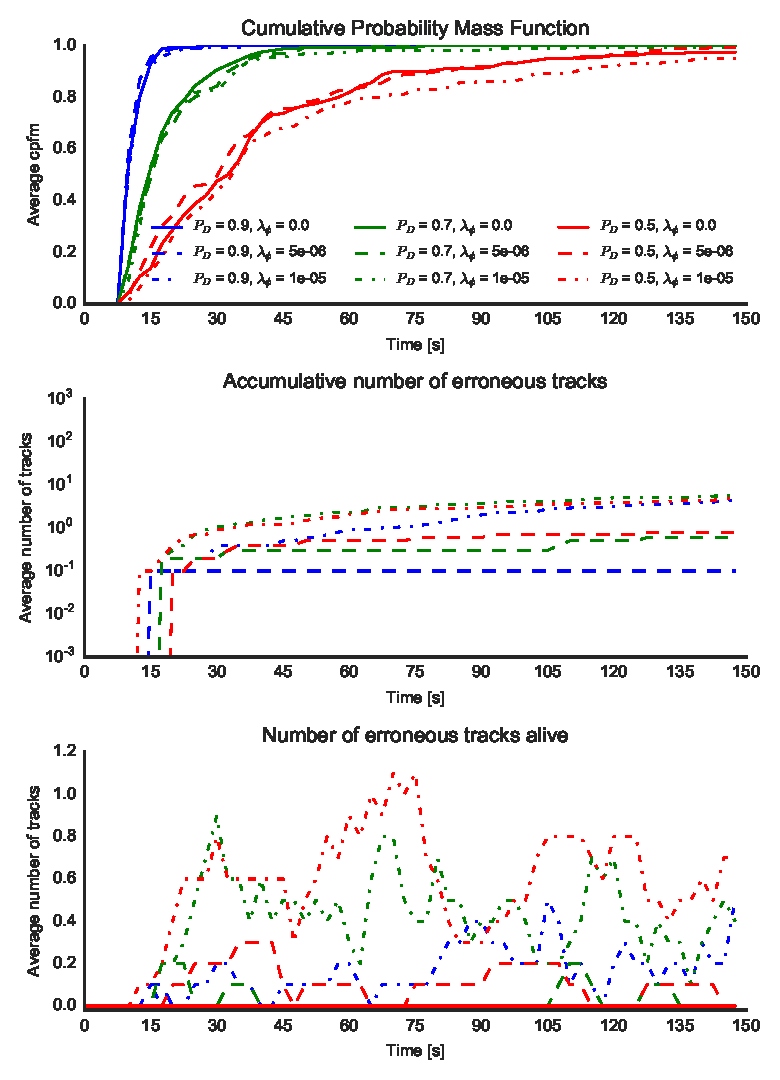
\includegraphics{Figures/plots/Scenario1_Init-Time(3-6).pdf}
\caption{Initialization time (3/6)}\label{fig:init_time_3-6}
\end{figure}